\input{preambuloSimple.tex}

%----------------------------------------------------------------------------------------
%	TÍTULO Y DATOS DEL ALUMNO
%----------------------------------------------------------------------------------------

\title{	
\normalfont \normalsize 
\textsc{\textbf{Ingeniería de Servidores (2016-2017)} \\ Grado en Ingeniería Informática \\ Universidad de Granada} \\ [25pt] % Your university, school and/or department name(s)
\horrule{0.5pt} \\[0.4cm] % Thin top horizontal rule
\huge Memoria Práctica 5 \\ % The assignment title
\horrule{2pt} \\[0.5cm] % Thick bottom horizontal rule
\begin{figure*}[!ht]
	\begin{center}
		\includegraphics[width=0.7\textwidth]{imagenes/escudo-de-la-universidad-de-granada}
	\end{center}
\end{figure*}
}

\author{Iván Rodríguez Millán} % Nombre y apellidos

\date{\normalsize\today} % Incluye la fecha actual

%----------------------------------------------------------------------------------------
% DOCUMENTO
%----------------------------------------------------------------------------------------

\begin{document}

\maketitle % Muestra el Título

\newpage %inserta un salto de página

\tableofcontents % para generar el índice de contenidos

\listoffigures

\listoftables

\newpage

\section{Al modificar los valores del kernel de este modo, no logramos que persistan después de reiniciar la máquina. ¿Qué archivo hay que editar para que los cambios sean permanentes?}
\subsection{Respuesta : }
Con el comando sysctl \cite{SYSCTL} podemos configurar parámetros del kernel mientras el sistema está corriendo. El único inconveniente es que al reiniciar el equipo, la configuración realizada con el comando se pierde. Para resolver este problema, podemos hacer los siguientes pasos que se mostrarán:

En primer lugar vamos a cambiar el valor del parámetro kernel.panic, que básicamente indica al sistema lo que debe esperar hasta reiniciarse cuando ocurra un kernel panic. Por defecto está a 0, nosotros lo cambiaremos a 5.

\begin{figure}[H]
	\begin{center}
		\includegraphics[width=15cm, height=1.5cm]{Imagenes/Indicando_valor_kernel_panic}
		\caption{Configurando el parámetro kernel.panic.}
		\label{fig:2}
	\end{center}
\end{figure}

Para que el cambio persista en el tiempo al reinicio del sistema, debemos ir al archivo de configuración ``/etc/sysctl.conf'' \cite{SYSCTL.CONF}, y añadir en el fichero el parámetro que queramos modificar con el valor que le vayamos a dar. Por ejemplo:

\begin{figure}[H]
	\begin{center}
		\includegraphics[width=15cm]{Imagenes/Anadiendo_valor_a_sysctl}
		\caption{Modificando un parámetro del fichero de configuración ``/etc/sysctl.conf''.}
		\label{fig:2}
	\end{center}
\end{figure}

Por último como se especifica en la documentación de sysctl para hacer efectivos los cambios tenemos el siguiente comando:

\begin{figure}[H]
	\begin{center}
		\includegraphics[width=15cm, height=1.5cm]{Imagenes/Sysctl_efectivos_cambios}
		\caption{Cargando los cambios realizados en el fichero sysctl.conf.}
		\label{fig:3}
	\end{center}
\end{figure}

\section{¿Con qué opción se muestran todos los parámetros modificables en tiempo de ejecución? Elija dos parámetros y explique, en dos líneas, que función tienen.}
\subsection{Respuesta : }
Para listar los parámetros modificables en tiempo de ejecución tenemos la opción sysctl -a. \cite{SYSCTL}

Para mostrar su uso, guardo la salida en un fichero para que sea mas fácil la visualización, ya que la salida es demasiado grande.

\begin{figure}[H]
	\begin{center}
		\includegraphics[width=15cm]{Imagenes/Uso_sysctl_a}
		\caption{Guardando la salida del comando sysctl -a.}
		\label{fig:4}
	\end{center}
\end{figure}

\begin{figure}[H]
	\begin{center}
		\includegraphics[width=15cm]{Imagenes/Mostrando_salida_sysctl}
		\caption{Fichero con la salida de sysctl -a.}
		\label{fig:5}
	\end{center}
\end{figure}

\begin{itemize}
	\item kernel.hostname: Permite cambiar el valor al nombre del equipo.
	\item kernel.hardlockup\_all\_cpu\_backtrace: Este parámetro controla el funcionamiento del detector de bloqueo duro, para que cuando se detecte un bloqueo duro, si se desea se pueda reunir mas información de depuración.
\end{itemize}
\newpage
\section{Realice una copia de seguridad del registro y restáurela, ilustre el proceso con capturas. Abra una ventana mostrando el editor del registro.}
\subsection{Respuesta : }

Para realizar la copia de seguridad del registro y posteriormente restaurarla hay dos opciones según \cite{RESTOREREGISTRY}, sacado de Microsoft. 
Una de estas dos opciones que se nos da es:

\begin{enumerate}
	\item Exportar el registro a algún lugar de nuestro PC.
	\item Importar ese registro previamente exportado.
\end{enumerate}

\begin{figure}[H]
	\begin{center}
		\includegraphics[width=15cm]{Imagenes/Exportacion_registro}
		\caption{Exportando el registro.}
		\label{fig:6}
	\end{center}
\end{figure}

\begin{figure}[H]
	\begin{center}
		\includegraphics[width=15cm]{Imagenes/Importacion_registro}
		\caption{Importando el registro.}
		\label{fig:7}
	\end{center}
\end{figure}

Pero al hacer todo este proceso, nos da un error al importar el registro.
\begin{figure}[H]
	\begin{center}
		\includegraphics[width=15cm]{Imagenes/Error_importacion}
		\caption{Error al importar el registro.}
		\label{fig:8}
	\end{center}
\end{figure}

Luego debemos escoger la opción de realizar un backup (Copia de seguridad del sistema). Para esto hay que hacer uso de una herramienta que no se encuentra instalada en nuestro servidor por defecto, es la conocida como Windows Server Backup \cite{INSTALACIONPOINTRESTORE}.

\begin{itemize}
	\item Para la instalación de esta herramienta seguimos los pasos de siempre para instalar servicios en nuestro Windows Server. Entramos a Server Manager - Manage - Add Roles and Features y una vez dentro seleccionamos la opcion Windows Server Backup y la instalamos (Todo el proceso de instalación no cambia con respecto a cualquier otra instalación de otro servicio que hayamos hecho en prácticas pasadas).
\end{itemize}

Cuando esté instalado, lo abrimos y nos encontraremos con algo similar a la imagen \ref{fig:9}.
 
\begin{figure}[H]
	\begin{center}
		\includegraphics[width=15cm]{Imagenes/Entrando_windows_server_backup}
		\caption{Pantalla de inicio del Windows Server Backup.}
		\label{fig:9}
	\end{center}
\end{figure}

Ahora el siguiente paso a tomar es realizar la copia de seguridad, y para esto es necesario irse a Backup Once, como se muestra en la imagen \ref{fig:9}.

A continuación se nos muestra el proceso por pasos:

\begin{figure}[H]
	\begin{center}
		\includegraphics[width=15cm]{Imagenes/Inicio_backup}
		\caption{Iniciando Backup en Windows Server Backup.}
		\label{fig:10}
	\end{center}
\end{figure}
\newpage
Elegimos si queremos una copia de todo el sistema o personalizada; en nuestro caso personalizada.
\begin{figure}[H]
	\begin{center}
		\includegraphics[width=15cm]{Imagenes/Indicando_backup_personalizado}
		\caption{Indicando Backup personalizado.}
		\label{fig:11}
	\end{center}
\end{figure}
\newpage
Elegimos los items que queremos guardar en nuestro backup.
\begin{figure}[H]
	\begin{center}
		\includegraphics[width=15cm]{Imagenes/Aniadimos_items_para_el_backup}
		\caption{Añadimos los items a copiar.}
		\label{fig:12}
	\end{center}
\end{figure}

\newpage
Posteriormente elegimos para guardar la copia de seguridad en local.
\begin{figure}[H]
	\begin{center}
		\includegraphics[width=15cm]{Imagenes/Indicando_donde_guardar_backup}
		\caption{Indicando donde guardar la copia de seguridad.}
		\label{fig:13}
	\end{center}
\end{figure}

\newpage
Seguidamente elegimos donde queremos guardar la copia, en nuestro caso pues elegimos una de las particiones libres.
\begin{figure}[H]
	\begin{center}
		\includegraphics[width=15cm]{Imagenes/Indicando_disk2.png}
		\caption{Indicando la partición donde guardar la copia de seguridad.}
		\label{fig:14}
	\end{center}
\end{figure}

\newpage
Después de este proceso nos aparecerá la siguiente imagen, indicándonos todas las características de la copia de seguridad que se llevará a cabo. Solo nos quedará darle a backup y el proceso finalizará.
\begin{figure}[H]
	\begin{center}
		\includegraphics[width=15cm]{Imagenes/Fin_1}
		\caption{Cuadro con todas las características del backup.}
		\label{fig:15}
	\end{center}
\end{figure}
\newpage

Tras este proceso de copia de seguridad, nos queda restaurar todos los datos previamente salvados correctamente. Para ello llevamos a cabo los siguientes pasos.

En primer lugar nos vamos a la pantalla de inicio de Windows Server Backup, y elegimos esta vez restore.
\begin{figure}[H]
	\begin{center}
		\includegraphics[width=15cm]{Imagenes/Seleccion_restore}
		\caption{Entrando en restore, para restaurar los datos previamente salvados.}
		\label{fig:16}
	\end{center}
\end{figure}
\newpage
En segundo lugar elegimos la restauración que queremos, en nuestro caso la ya mencionada anteriormente.
\begin{figure}[H]
	\begin{center}
		\includegraphics[width=15cm]{Imagenes/Indicando_punto_restauracion}
		\caption{Elegimos el punto de restauración que deseamos realizar.}
		\label{fig:17}
	\end{center}
\end{figure}

\newpage
Tras darle a siguiente nos pedirá confirmación y le damos a que deseamos continuar.
\begin{figure}[H]
	\begin{center}
		\includegraphics[width=15cm]{Imagenes/Inicio_restauracion}
		\caption{Iniciando restauración.}
		\label{fig:18}
	\end{center}
\end{figure}

\newpage
Después nos saldrá una pantalla con el proceso de restauración con todo lujo de detalles. Una vez que finalice dicho paso, el sistema se reiniciará para finalizar con todo el proceso.
\begin{figure}[H]
	\begin{center}
		\includegraphics[width=15cm]{Imagenes/Estado_restauracion}
		\caption{Proceso de restauración.}
		\label{fig:19}
	\end{center}
\end{figure}

\newpage
Tras el reinicio se nos mostrará un cmd (símbolo del sistema) indicándonos que todo a salido satisfactoriamente, y solo tendremos que pulsar en ENTER para continuar, y dar por finalizado el proceso de restauración.
\begin{figure}[H]
	\begin{center}
		\includegraphics[width=15cm]{Imagenes/Fin_restauracion}
		\caption{Finalización del proceso de restauración.}
		\label{fig:20}
	\end{center}
\end{figure}

\newpage
Por último se nos pide que mostremos una imagen con el editor de registro (registry editor) abierto. En mi caso lo he hecho dirigiéndome a ``search''(Buscador de Windows) y buscándolo por regedit. Aunque también podemos ir al cmd y poner regedit, y se nos abrirá el editor.

\begin{figure}[H]
	\begin{center}
		\includegraphics[width=15cm]{Imagenes/Editor_registro}
		\caption{Editor de registro de Windows.}
		\label{fig:21}
	\end{center}
\end{figure}

\newpage
\section{Enumere qué elementos se pueden configurar en Apache y en IIS para que Moodle funcione mejor.}
\subsection{Respuesta : }

Para Apache :

\begin{itemize}
	\item Ajustar la directiva ``MaxClients'' en función de la memoria disponible. Nos facilitan una fórmula:
	\begin{figure}[H]
	\begin{center}
		\includegraphics[width=15cm]{Imagenes/MaxClients}
		\caption{Configuración de la sentencia de MaxClients.}
		\label{fig:22}
	\end{center}
\end{figure}

	\item Reducir el número de módulos que Apache carga en el archivo httpd.conf al mínimo necesario para reducir la memoria necesaria.
	\item Utilizar la última versión de Apache.
	\item Reducir el ``MaxRequestsPerChild'' hasta 20-30.
	\item Si el servidor estuviese muy cargado, bajar el KeepAlive Timeout sobre 2-5. Cuanto mayor sea el valor más procesos del servidor se mantendrán esperando conexiones posiblemente inactivas. Un valor más exacto para KeepAliveTimeout se obtiene observando cuánto tiempo tarda sus usuarios en descargar una página. Después de alterar cualquiera de las variables de KeepAlive, supervise la utilización de la CPU, ya que puede haber una sobrecarga adicional al iniciar más procesos / sub-procesos de trabajo.
	\item Considerar la posibilidad de configurar un servidor Proxy inverso delante del servidor Moodle para almacenar en caché archivos HTML con imágenes.
	\item En caso de no utilizar un archivo .htaccess, se recomienda establecer la variable AllowOverride en AllowOverride None para evitar las búsquedas de .htaccess.
	\item Establecer el DirectoryIndex correctamente para evitar la negociación de contenido.
	\item Cuando no se esté realizando trabajos de desarrollo en el servidor, se recomienda establecer ExtendedStatus desactivado y deshabilitar mod\_info así como mod\_status.
	\item Dejar HostnameLookups desactivado para reducir la latencia del DNS.
	\item Consider reducing the value of TimeOut to between 30 to 60 (seconds).
	\item Reducir el valor de TimeOut a entre 30 y 60 (segundos).
	\item La compresión reduce los tiempos de respuesta, reduciendo los tamaños de la respuesta HTTP.
\end{itemize}

Para IIS:
\begin{itemize}
	\item Establecer el ListenBackLog que es el equivalente a KeepAliveTimeout, entre los valores 2 y 5.
	\item Cambiar el valor MemCacheSize para ajustar la cantidad de memoria (Mb) que IIS utilizará para su caché de archivos.
	\item Cambiar el valor MaxCachedFileSize para ajustar el tamaño máximo de un archivo almacenado en caché en el caché de archivos en bytes. El valor predeterminado es 262.144 (256K).
	\item Crear un nuevo DWORD llamado ObjectCacheTTL para cambiar la longitud de tiempo que los objetos en el caché se almacenan en memoria.
\end{itemize}
\newpage
\section{Ajuste la compresión en el servidor y analice su comportamiento usando varios valores para el tamaño de archivo a partir del cual comprimir. Para comprobar que está comprimiendo puede usar el navegador o comandos como curl o linx. Muestre capturas de pantalla de todo el proceso.}
\subsection{Respuesta : }

Para habilitar la compresión nos vamos al símbolo del sistema (cmd), una vez dentro nos dirigimos a la ruta /windows/system32/inetsrv, tras este paso pasamos a habilitar los tipos de compresión dinámico y estático: \cite{HABILITARCOMPRESION}

\begin{itemize}
	\item appcmd set config /section:urlCompression /doStaticCompression:True
	\item appcmd set config /section:urlCompression /doDynamicCompression:True
\end{itemize} 

\begin{figure}[H]
	\begin{center}
		\includegraphics[width=15cm]{Imagenes/Activacion_compresion_statica_dinamica}
		\caption{Habilitando compresion para IIS.}
		\label{fig:23}
	\end{center}
\end{figure}

Después de este proceso, pasaremos a configurar las características de la compresión desde el panel de IIS manager. En donde puedes por ejemplo establecer la barrera a partir de la cual se empieza a realizar compresión (En nuestro caso será de 256 bytes).

\begin{figure}[H]
	\begin{center}
		\includegraphics[width=15cm]{Imagenes/Configuracion_compresion}
		\caption{Habilitando compresion para IIS.}
		\label{fig:24}
	\end{center}
\end{figure}

Para mostrar un ejemplo de compresión, realizamos una petición a la página de la UGR \cite{UGR}, y con la herramienta disponible para Google Chrome denominada ``HTTP Headers'' mostramos las cabeceras de las peticiones y respuestas de la página.

\begin{figure}[H]
	\begin{center}
		\includegraphics[width=15cm]{Imagenes/Probando_compresion}
		\caption{Probando si la página web de la UGR realiza compresión.}
		\label{fig:25}
	\end{center}
\end{figure}

Vemos como en el campo accept-encoding de la solicitud se indican los tipos de compresión por parte del cliente (gzip, deflate, sdch, br) y más abajo se puede visualizar el tipo de compresión que ha realizado el servidor (gzip) en el campo content-encoding.
\newpage
\section{Usted parte de un SO con ciertos parámetros definidos en la instalación, ya sabe instalar servicios y cómo monitorizarlos cuando los somete a cargas. Al igual que ha visto cómo se puede mejorar un servidor web, elija un servicio y modifique un parámetro para mejorar su comportamiento. Monitorice el servicio antes y después de la modificación del parámetro aplicando cargas al sistema mostrando los resultados de la monitorización.}
\subsection{Pruebas : }
Para este apartado, llevaré a cabo una comparativa de dos sistemas de archivos bastante conocidos, como son Ext3 y Ext4. La motivación que me llevó a realizar el ejercicio sobre los sistemas de archivos ha sido principalmente el querer comprobar por uno mismo, si, lo que se habla en algunos estudios realizados por empresas (que comentaremos más adelante) es definitivo para, a la hora de escoger uno u otro acertemos.

Uno de los estudios que van en mayor profundidad que he visto en internet ha sido el realizado por RedHat \cite{REDHATESTUDIO}.
\\
También saqué información en cuanto a los sistemas de archivos en Ubuntu de \cite{FILESYSTEM}, en donde se nos habla de conceptos como el de journaling o fragmentación.
\\
Haciendo un muy breve resumen de los datos proporcionados por el último enlace mencionado, sale lo siguiente:

\begin{table}[H]
\centering
\begin{tabular}{|l|c|c|c|c|}
\hline
\textbf{Sistema Archivos} & \textbf{Tamaño Archivo} & \textbf{Tamaño Partición} & \textbf{Journaling}\\
\hline
Ext3 & 2TiB & 32 TiB & Sí\\
\hline
Ext4 & 16TiB & 1 EiB & Sí\\
\hline
\end{tabular}  
\caption{Tabla comparativa de Ext3 y Ext4.} 
\label{tab:1}
\end{table}

Para comprobar el rendimiento de dos servidores con diferentes sistemas de archivos vamos a realizar dos pruebas diferentes, por un lado haremos un estrés de disco usando un test de Phoronix Suite, este test es conocido como AIO-Stress. \cite{AIOSTRESS}
\\
Y por otro lado lanzaremos en cada máquina un script realizado en Python que básicamente calcula el tiempo que se tarda en : Crear un directorio, crear un número definido por nosotros de ficheros con un tamaño también definido por nosotros, escribir en cada fichero, leer de forma linear de cada fichero, leer de forma aleatoria de cada fichero y eliminar todos estos ficheros.

\newpage
Para el caso de usar Phoronix Suite:

\begin{itemize}
	\item En una máquina con Ext3 como sistema de archivos:
\end{itemize}

Tenemos una media de 66.34 MB/s de escritura aleatoria con una desviación típica de 4.87. \cite{BENCHMARKPHORONIXEXT3}
\begin{figure}[H]
	\begin{center}
		\includegraphics[width=15cm]{Imagenes/Estres_ext3}
		\caption{Test de Phoronix Suite.}
		\label{fig:26}
	\end{center}
\end{figure}

\begin{itemize}
	\item En una máquina con Ext4 como sistema de archivos:
\end{itemize}

Tenemos una media de 106.84 MB/s de escritura aleatoria con una desviación típica de 6.59. \cite{BENCHMARKPHORONIXEXT4}
\begin{figure}[H]
	\begin{center}
		\includegraphics[width=15cm]{Imagenes/Estres_ext4}
		\caption{Test de Phoronix Suite.}
		\label{fig:27}
	\end{center}
\end{figure}

Para una primera conclusión breve (Ya que después se hará una más profunda) sobre los test, podemos deducir que la máquina con el sistema de archivos Ext4 llega casi a doblar en MB/s a la máquina con Ext3, lo cual ya nos indica una mejora sustancial como para elegir entre uno u otro.

\newpage
Pero aunque veamos unos datos con diferencias bastante grandes usando Phoronix Suite, se ha realizado un script en Python algo más completo, para comprobar con creación de ficheros, eliminación de ficheros, lectura tanto aleatoria como secuencial, si en realidad la diferencia es tan grande, o Ext3 se aproxima algo a los resultados de Ext4.

Para el caso de creación de un directorio:

\begin{figure}[H]
	\begin{center}
		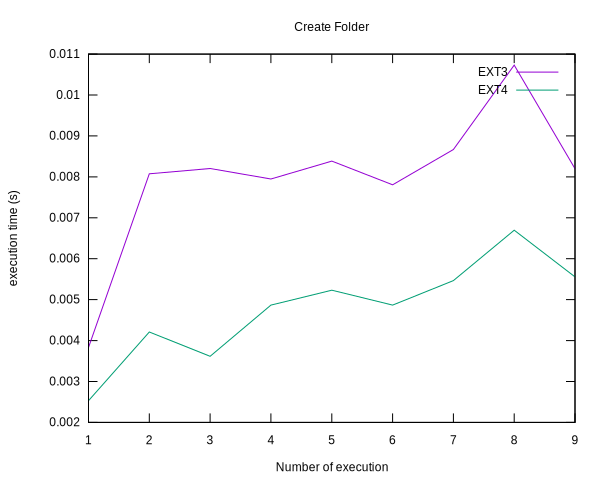
\includegraphics[width=15cm]{Imagenes/CreateFolder}
		\caption{Gráfica de los resultados de crear un directorio con dos máquinas con sistemas de archivos diferentes.}
		\label{fig:28}
	\end{center}
\end{figure}

En el caso de la creación de un directorio donde después crearemos los diferentes ficheros que indiquemos, gana la máquina con ext4 como sistema de archivos.
\newpage
Para el caso de creación de los varios ficheros con tamaño de 1024 Bytes cada uno:

\begin{figure}[H]
	\begin{center}
		\includegraphics[width=15cm]{Imagenes/Create_Files}
		\caption{Gráfica de los resultados de crear varios ficheros con dos máquinas con sistemas de archivos diferentes.}
		\label{fig:29}
	\end{center}
\end{figure}

Para el caso de crear los ficheros, cada fichero tiene un tamaño de 1024 Bytes (1KB). Se ve como se producen dos picos uno por parte de ext3 y otro por parte de ext4, pero por lo demás son tiempos similares.

\newpage
Para el caso de escribir en los ficheros :

\begin{figure}[H]
	\begin{center}
		\includegraphics[width=15cm]{Imagenes/Write_Files}
		\caption{Gráfica de los resultados de escribir en los ficheros con dos máquinas con sistemas de archivos diferentes.}
		\label{fig:30}
	\end{center}
\end{figure}

Aquí vemos como ext3 se comporta mejor que ext4, !justo lo contrario que ocurría usando el test de Phoronix Suite¡, aunque si que es verdad que en este caso las diferencias son mínimas, mientras que en Phoronix Suite eran mayores. Mucho cuidado porque en Phoronix Suite se miden MB/s y aquí segundos, por ello quiero dejar claro que a la hora de comparar ambos tiempos hay que tener cuidado.

\newpage
Para el caso de la lectura de forma lineal de los diferentes ficheros:

\begin{figure}[H]
	\begin{center}
		\includegraphics[width=15cm]{Imagenes/Read_Files_Linear}
		\caption{Gráfica de los resultados de leer de forma lineal de los diferentes ficheros con dos máquinas con sistemas de archivos diferentes.}
		\label{fig:31}
	\end{center}
\end{figure}

Para el caso de la lectura lineal se ve que al comienzo con un número reducido de ficheros ext3 se comporta algo mejor, pero conforme el número de ficheros va creciendo, se van igualando los tiempos.

\newpage
Para el caso de la lectura de forma aleatoria de los diferentes ficheros:

\begin{figure}[H]
	\begin{center}
		\includegraphics[width=15cm]{Imagenes/Read_Files_Random}
		\caption{Gráfica de los resultados de leer de forma aleatoria de los diferentes ficheros con dos máquinas con sistemas de archivos diferentes.}
		\label{fig:32}
	\end{center}
\end{figure}

Cuando se lee de forma aleatoria se ve que prácticamente es similar, salvo este pico que hace hacia abajo la máquina con ext3, al que habría que restarle importancia.

\newpage
Para el caso de eliminar los ficheros previamente creados y el directorio:

\begin{figure}[H]
	\begin{center}
		\includegraphics[width=15cm]{Imagenes/Delete_Files}
		\caption{Gráfica de los resultados de eliminar los ficheros previamente creados con dos máquinas con sistemas de archivos diferentes.}
		\label{fig:33}
	\end{center}
\end{figure}

En el caso de la eliminación de lo que se ha ido creando, los resultados son similares.
\newpage
\subsection{Conclusión}

Antes de concluir con un resumen de lo ocurrido en los test hay que despejar ciertas incógnitas con respecto a las ventajas que acarrea tener ext4 frente a ext3:
\begin{itemize}
	\item En ext3 solamente se pueden alojar 32000 subdirectorios, mientras que en ext4 no hay límite.
	\item Delayed allocation por parte de ext4, puede retrasar la escritura en disco hasta el último momento.
	\item Aunque ext3 no es propenso a la fragmentación excesiva, los archivos almacenados en si es probable que se fragmenten. Ext4 agrega soporte para la des-fragmentación en línea, con lo que debería de mejorar el rendimiento general. 
\end{itemize}

Estas son algunas de las ventajas de ext4 sobre ext3.
\\
Con respecto a lo ocurrido en los test, si que es verdad que en el caso de Phoronix Suite se ha visto una gran diferencia de rendimiento, algo que es normal puesto que ext4 es una mejora con respecto a ext3, aunque también debemos tener en cuenta estas últimas gráficas en donde los tiempos son similares. 
\\
Si yo tuviese que elegir después de todo un sistema de archivos, obviamente utilizaría Ext4, a parte de por las mejoras de las que hablan las empresas como IBM \cite{FILESYSTEMIBM}, Ubuntu \cite{FILESYSTEM} ó el mismo REDHAT \cite{REDHATESTUDIO} con un análisis bastante más profundo, también fijándonos en los resultados de nuestros tests.
\newpage
\bibliography{citas} %archivo citas.bib que contiene las entradas 
\bibliographystyle{ieeetr} % hay varias formas de citar

\end{document}
